\tightsection{Prediction algorithms}
\label{prediction}
The tradeoff between estimation error and bias via aggregation naturally leads us to consider a class of algorithms that compute average quality outcomes for groups of sessions under different attribute sets, and then {\it dynamically} choose the attribute set that seems to work well for a particular session under prediction.  Since it is difficult to find the best attribute set, it is useful to hedge our bets by taking a weighted combination of averages.  George et al \cite{george2008value} consider this problem and propose the following algorithm for choosing the weights.  For a session under prediction having index $i$, let $a_i$ be the tuple of all attributes observed for that session and let $q_i$ be its quality outcome.  For each attribute set $g$ in our collection of attribute sets $G$, define a function $v_g$ that picks out those attributes:
\begin{equation*}
  v_g(\cdot): a \mapsto \text{[the subtuple of $a$ containing attribute values for the attributes in g]} .
\end{equation*}
We first compute the single-group average quality outcome for each $g$:
\begin{align*}
  \bar{q}_{g}(a_i) &= \frac{1}{N_{g}(a_i)} \sum_{j \in N_{g}(a_i)} q_j, \text{ where} \\
  N_{g}(a_i) &= |\{j: v_g(a_j) = v_g(a_i), j < N\}|
\end{align*}
Then, considering $\bar{q}_{g}(a_i)$ as an estimate of $q_i$, estimate its mean squared prediction error $e_{g}(a_i)$.  This estimation step is not simple, so we will briefly postpone its description.  Having computed $\bar{q}_{g}(a_i)$ and $e_{g}(a_i)$ for each attribute set, our final quality prediction, which we denote $\bar{q}(a_i)$, is the weighted average of $\bar{q}_{g}(a_i)$, where the weights are equal to the inverse of $e_{g}(a_i)$, normalized to sum to $1$:
\begin{align*}
  \bar{q}(a_i) = (\sum_{g \in G} e_{g}(a_i)^{-1})^{-1} \sum_{g \in G} e_{g}(a_i)^{-1} \bar{q}_{g}(a_i) .
\end{align*}

$e_{g}(a_i)$ is estimated by separately estimating (squared) bias and estimation error and summing them, plugging them into equation \eqref{eqn:biasvariance}.  Bias is heuristically taken to be the difference between the finest-granularity estimate of $q_i$ (i.e. $\bar{q}_{g'}(a_i)$, where $g'$ is the finest-grained ACS) and $\bar{q}_{g}(a_i)$.  Variance is estimated by a standard formula:
\begin{align*}
  \frac{1}{N_{g}(a_i)} \sum_{j \in N_{g}(a_i)} (q_j - \bar{q}_{g}(a_i))^2
\end{align*}

George et al call the resulting prediction algorithm WIMSE, for Weighted Inverse Mean Squared Error.  Inverse-mean-squared-error weighting has the following nice property: If each $\bar{q}_{g}(a_i)$ is statistically independent, then $\bar{q}$ is an optimal estimator in the sense that it has minimal mean squared error among all functions of \cite{}.  However, in our setting (and in the original motivating setting) the $\bar{q}_{g}(a_i)$ are based on overlapping data and are therefore not independent.  Further, our estimates of both the bias and variance components of $e_{g}(a_i)$ are imprecise.  Thus we have no neat theoretical guarantee of optimality for WIMSE.  George et al find that WIMSE can nevertheless work well.  The deficiencies of the algorithm necessitate a few tweaks in our setting, which we now present.

\begin{figure*}[t!]
\centering
\subfigure[Exhaustive vs. greedy (GO) search]
{
        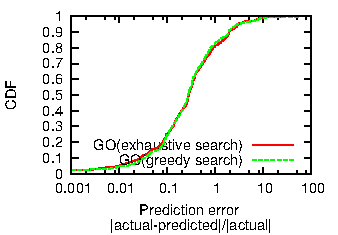
\includegraphics[width=0.3\textwidth]{figures/prediction-comparisons/example-exhaustive-metric1.pdf}
}
\subfigure[GO vs. variants]
{
        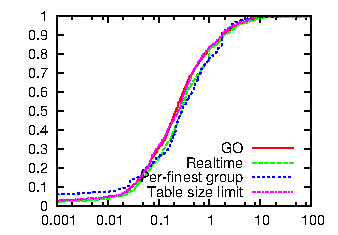
\includegraphics[width=0.3\textwidth]{figures/prediction-comparisons/example-acs-metric1.pdf}
}
\subfigure[GO vs. oracle (optimal AC)]
{
        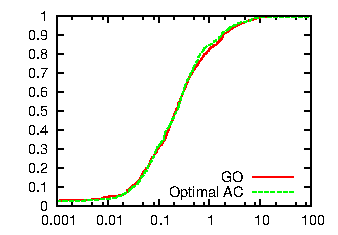
\includegraphics[width=0.3\textwidth]{figures/prediction-comparisons/example-oracle-metric1.pdf}
}
\tightcaption{Comparison between GO ACS selection with other strawmans (considerd quality metric is average bitrate).}
\label{fig:acs-comparison}
\end{figure*}

\tightsubsection{ACS selection}

\myparasum{Why ACS selection instead of the full ACS?} One statistical reason is that with more ACs, WIMSE does not necessarily perform better. In fact, \jc{Henry, \fillme} Another practical reason is that to store groups of all possible values of all possible ACs, the memory requirement will be prohibitively high, which will be a potential bottleneck of the whole system as \Section~\ref{sec:scalability}. 

\myparasum{Greedy static ACS selection and strawmans} We take a data-driven approach to ACS selection. We separate part of historical sessions as test set and best ACS selection is the one that gives the best average accuracy over the test set using WIMSE. 

\myparasum{Justify greedy algorithm} One problem with this approach is that even in offline analysis, the potential space to search for the best ACS is too huge (with $k$ attributes, there will be $2^k$ ACs, and in total $2^{2^k}$ ACSes). Instead, we first examine a greedy algorithm which find a good ACS in $O(2^k)$ amount of steps, and compare it against exhaustive search result with $k=3$ attributes (i.e., 256 ACSes). Figure~\ref{fig:acs-comparison}-(a) presents the CDF of prediction accuracy w.r.t average bitrate of the ACS that obtained by exhaustive search and greedy search. It shows that the ACS they choose, though different, can offer similar quality of prediction.

\jc{Pseudo code of greedy ACS selection.}

\myparasum{Per-finest group selection vs. one global ACS} One strawman for our algorithm to compare with is one where the selected ACS can be different for different sessions. Especially, if two sessions differ in at least one attribute, they can use different ACS. \fillme. \jc{Results shown in Figure~\ref{fig:acs-comparison}-(b), and they perform similarly and the global ACS performs even slightly better, possibly because per-finest-group ACS has side-effect of overfitting.}

\myparasum{Oracle approach vs. historical based} \fillme. \jc{Results shown in Figure~\ref{fig:acs-comparison}-(b). Result needs to be changed after discussion today.}

\tightsubsection{Pseudocount priors}
That algorithm assumes that bias and variance can be computed exactly, while in practice variance cannot be estimated accurately when groups are very small.  To alleviate this, we use a simple idea from Bayesian statistics: We incorporate a prior distribution on quality outcomes within each group.  This amounts to adding a few fake ``pseudocount'' observations to each group.  \fillme.


\begin{figure}[h!]
\centering
 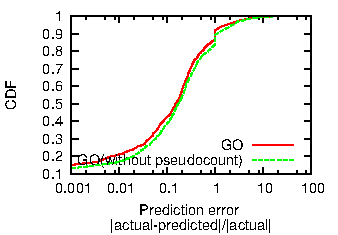
\includegraphics[width=0.4\textwidth] {figures/prediction-comparisons/example-pcount-metric1.pdf}
\tightcaption{GO with pseudocount vs. without pseudocount (considerd quality metric is average bitrate).}
\label{fig:quality-variability}
\end{figure}

For each of these we should have a CDF of errors and also the average prediction error.
\begin{itemize}
	\item GO with greedy ACS selection and pseudocount priors
	\item GO with greedy ACS selection and no pseudocounts
\end{itemize}

\tightsubsection{Mini-evaluation of prediction accuracy}
Given an ACS selection algorithm, we’re going to use all attributes we have and test GO prediction accuracy against two simple baselines.
\begin{itemize}
	\item GO with greedy ACS selection and pseudocount priors
	\item Predict using average of last 2 hours on all traffic for this CDN
	\item Predict using average of last 2 hours on the finest group that has any data
\end{itemize}
For each of these we should have a CDF and also display the average prediction error.

\begin{figure*}[t!]
\centering
\subfigure[Buffering ratio]
{
        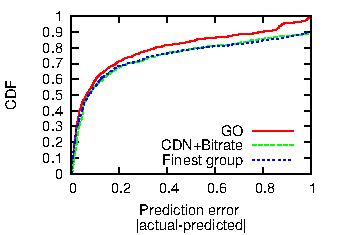
\includegraphics[width=0.22\textwidth]{figures/prediction-comparisons/example-naive-metric0.pdf}
}
\subfigure[Average bitrate]
{
        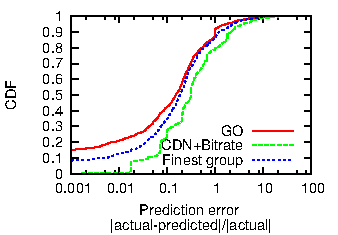
\includegraphics[width=0.22\textwidth]{figures/prediction-comparisons/example-naive-metric1.pdf}
}
\subfigure[Join time]
{
        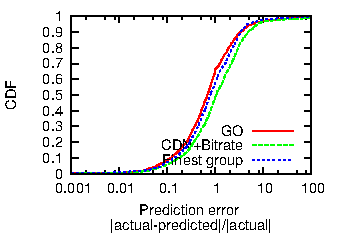
\includegraphics[width=0.22\textwidth]{figures/prediction-comparisons/example-naive-metric2.pdf}
}
\subfigure[Start failure]
{
        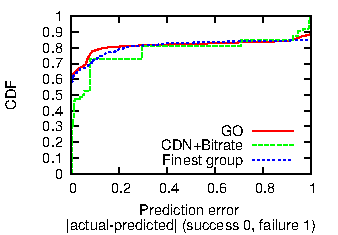
\includegraphics[width=0.22\textwidth]{figures/prediction-comparisons/example-naive-metric3.pdf}
}
\tightcaption{Comparison between GO and two baseline approaches where the selection and use of ACS is statically used -- (1) no attributes considered except (CDN, bitrate), (2) all attributes considered.}
\label{fig:compare-to-naive}
\end{figure*}

\henry{The following two subsections contain a bunch of caveats.  It might be more effective to move them to a later section on future work.}

\tightsubsection{Interactions between decisions}
The reader may be bothered by a simplifying assumption implicit in our characterization of the causes of prediction error.  If we allocated all traffic to a single CDN, its performance might degrade, but our session-wise prediction does not capture that.  We might instead want to know the following: Given a set of decisions about sessions (say, all the sessions we observe in a 1-hour interval), what is the predicted performance for that set of sessions?  We do not wish to say that such a question is impossible to answer, but rather point out some difficulties in answering it, and some reasons why it is less critical to answer it than it may appear.

Joint prediction is statistically difficult because existing statistical prediction algorithms typically assume the performance of training examples are independent and experience identical randomness (i.e. they are IID).  We observe very few IID instances of whole sets of sessions; in our example, we observe only one per 1-hour interval.  It is possible to model explicitly the dependence of each session’s performance on the set of joint decisions, but this requires modeling choices that we may not make well, and such models are typically computationally expensive to learn. \fillme

If conditions change slowly enough, the independence assumption is not so bad.
The rate of change of CDN allocations is naturally limited for our problem by the rate of session arrivals, since we choose CDNs only at the beginning of each session.  Spikes in the rate of new sessions are not typically high enough to necessitate special handling.  \henry{Need some data and experiments for this.  Davis or Florin have done some of the experiments, I think.}

\tightsubsection{Alternative approaches}
The reader should not leave with the impression that the algorithm described above is the only possible one for predicting video quality, or even the best.  The scope of this paper is merely to establish a reasonable approach and show that it results in improvements.  Other possible approaches might include:
\begin{packedenumerate}
  \item \emph{Linear regression:} After encoding categorical attributes as binary features, simple linear regression can be applied to predict quality outcomes.  Temporal attributes can be passed through nonlinear functions to achieve reasonable time-series prediction.  Interaction terms (e.g. the indicator for a session coming from ASN $100$ multiplied by the indicator for the session having Object ``foo'') can simulate attribute combinations, at the cost of a combinatorial explosion in the size of the learned model.  However, recent developments in optimization for $\ell_1$-regularized linear regression allow models to be learned quickly online while providing the guarantee that the learned model is \emph{sparse}, i.e. that only a few important features are selected for inclusion in the model and the rest can be safely dropped.  See \cite{duchi2010composite} for one example of work that could enable this technique.  One downside is that linear models are harder to interpret than a model based on averaging group averages.
  \item \emph{Hierarchical Bayesian modeling:} In this approach, groups are placed in the natural tree, and each is associated with a probability distribution over quality outcomes, such as a Gaussian distribution.  Each group inherits information from the distribution of its parent group in the form of a prior.  Such models potentially deal very naturally with data sparsity and with dependence among sessions \cite{gelman2003bayesian}, but learning them from data is often computationally intractable.
\end{packedenumerate}